\documentclass[conference]{IEEEtran}
\IEEEoverridecommandlockouts
\usepackage{fancyhdr}
\usepackage[english]{babel}

% Phil's macros
% Create code font alias
\usepackage{tikz}
% Code
\usepackage{listings}
\usepackage{xcolor}
\newcommand{\code}[1]{\texttt{#1}}
\usepackage{minted}
\usepackage{algorithm}
\usepackage{standalone}
\usepackage{algorithmicx}
\usepackage[noend]{algpseudocode}
\usemintedstyle{trac}
\renewcommand\algorithmicdo{}
\renewcommand\algorithmicthen{}
\setlength{\parindent}{0em}

\pagestyle{fancy}
\fancyhead{}

\lstdefinestyle{customc}{
belowcaptionskip=1\baselineskip,
breaklines=true,
frame=L,
xleftmargin=\parindent,
language=C,
showstringspaces=false,
basicstyle=\footnotesize\ttfamily,
keywordstyle=\bfseries\color{green!40!black},
commentstyle=\itshape\color{purple!40!black},
identifierstyle=\color{blue},
stringstyle=\color{orange},
columns=fullflexible,
language=c,
frame=true,
numbers=left
}
\lstdefinestyle{snippet}{
belowcaptionskip=1\baselineskip,
breaklines=true,
frame=L,
xleftmargin=\parindent,
language=C,
showstringspaces=false,
basicstyle=\footnotesize\ttfamily,
keywordstyle=\bfseries\color{green!40!black},
commentstyle=\itshape\color{purple!40!black},
identifierstyle=\color{blue},
stringstyle=\color{orange},
columns=fullflexible,
language=c
}
\lstdefinestyle{hex}{
belowcaptionskip=1\baselineskip,
breaklines=true,
frame=LR,
% xleftmargin=\parindent,
language=C,
showstringspaces=false,
basicstyle=\footnotesize\ttfamily,
keywordstyle=\bfseries\color{green!40!black},
commentstyle=\itshape\color{purple!40!black},
% identifierstyle=\color{blue},
stringstyle=\color{orange},
columns=fullflexible,
keywords=[2]{fail},
keywords=[3]{pass},
keywordstyle={\color{blue!80!black}},
keywordstyle=[2]{\color{red!80!black}},
keywordstyle=[3]{\color{green!50!black}},
}

\lstdefinestyle{asm}{
belowcaptionskip=1\baselineskip,
keepspaces,
breaklines=true,
tabsize=8,
frame=L,
xleftmargin=\parindent,
language=[x86masm]Assembler,
showstringspaces=false,
basicstyle=\footnotesize\ttfamily,
keywordstyle=\bfseries\color{green!40!black},
commentstyle=\itshape\color{purple!40!black},
identifierstyle=\color{blue},
stringstyle=\color{orange},
columns=fullflexible,
}

% The preceding line is only needed to identify funding in the first footnote. If that is unneeded, please comment it out.
\usepackage{cite}
\usepackage{amsmath,amssymb,amsfonts}
\usepackage{graphicx}
\usepackage{textcomp}
\def\BibTeX{{\rm B\kern-.05em{\sc i\kern-.025em b}\kern-.08em
T\kern-.1667em\lower.7ex\hbox{E}\kern-.125emX}}
\begin{document}

\title{Breaking Trivium with Stuck-at-0 Faults}

\author{\IEEEauthorblockN{Phillip Gajland}
\IEEEauthorblockA{\textit{KTH Royal Institute of Technology} \\
\textit{Theoretical Computer Science} \\
Stockholm, Sweden \\
gajland@kth.se}
\and
\IEEEauthorblockN{Daniel Skantz}
\IEEEauthorblockA{\textit{KTH Royal Institute of Technology} \\
\textit{Theoretical Computer Science} \\
Stockholm, Sweden \\
danska@kth.se}
\and
\IEEEauthorblockN{Elena Dubrova}
\IEEEauthorblockA{\textit{KTH Royal Institute of Technology} \\
\textit{Electronic Systems Design} \\
Stockholm, Sweden \\
dubrova@kth.se}
}

\maketitle

\begin{abstract}
As the Internet of Things (IoT) continues to gain traction, so does the need for secure IoT devices. Although 23.3 billion IoT devices are estimated to be connected by 2023 \cite{iot}, vendors often neglect the security of such devices. Stream ciphers can offer an attractive solution for secure communications, when low power consumption is essential. 

The eSTREAM project was intended to \textit{"identify new stream ciphers suitable for widespread adoption"}.\cite{call} In 2018, Trivium, a synchronous stream cipher was selected as part of the portfolio for low area hardware ciphers. 

In this paper we study the design choices made by the authors of Trivium in order to demonstrate a fault attack on the software implementation of the cipher. Whilst Trivium maintains most desirable cryptographic properties, a simple design was chosen by the authors to provide flexibility. Our attack works by modifying the compiled binary at targeted positions to introduce stuck at 0 faults. Using this technique, we are able to reduce the non-linear feedback function to a linear one. Thus, it is possible to recover the 288-bit internal state of the cipher. In turn extraction of the 80-bit key becomes tractable.
\end{abstract}

\begin{IEEEkeywords}
trivium, stream cipher, fault attack
\end{IEEEkeywords}

\section{Introduction}

As the Internet of Things (IoT) continues to gain traction, so does the need for secure IoT devices. Although 23.3 billion IoT devices are estimated to be connected by 2023 \cite{iot}, vendors often neglect the security of such devices. Stream ciphers can offer an attractive solution for secure communications, when low power consumption is essential.




In this paper we analyse the design choices made by the authors of Trivium, in order to discover a new class of vulnerabilities. 


We go on to demonstrate a fault attack on the software implementation of Trivium.



The eSTREAM project was intended to \textit{"identify new stream ciphers suitable for widespread adoption"}.\cite{call} In 2018, Trivium, a synchronous stream cipher was selected as part of the portfolio for low area hardware ciphers. In this paper we analyse the design choices made by the authors of Trivium. We go on to demonstrate a fault attack on the software implementation of Trivium. 

The attack works by modifying compiled binaries at targeted positions to introduce stuck at 0 faults. Using this technique, we are able to reduce the non-linear feedback function to a linear one. Thus, it is possible to recover the 288-bit internal state of the cipher and in turn extraction of the 80-bit key becomes tractable.


trade off between performance and security, when low power consumption is of high significance. 


Stream ciphers can offer an attractive trade off between security and per in situations where power consutmption 
, due to their low


When performance 

A primary concern is securing systems 

an attractive solution when low powerconsumption is vital 
Thus, significantly increasing the attack surface for adversaries to mount attacks on larger systems, as was demonstrated in the 2016 Dyn cyberattack.


Stream Ciphers offer an attractive trade-off between lightweight crypto primitives and security in 


\begin{itemize}
\item[$\blacktriangleright$] A network is only as secure as its weakest link.
\item[$\blacktriangleright$] 23.3 billion IoT devices by 2023.
\item[$\blacktriangleright$] Need for securing IoT devices.
\begin{itemize}[itemsep=0.25cm]
\item[$\triangleright$] DDoS attacks e.g. Dyn cyberattack 2016.
\end{itemize}
\item[$\blacktriangleright$] Require energy efficient ciphers.
\end{itemize}

\section{Background}

As a result of the failures of all six stream ciphers submitted to the NESSIE (New European Schemes for Signatures, Integrity and Encryption) project, the eSTREAM project was launched in 2004 in order to \textit{"identify new stream ciphers suitable for widespread adoption"} \cite{call}. As a result, a portfolio of new stream ciphers was announced in April 2008. The portfolio was revised in September 2008, and currently consist of seven stream ciphers.

\begin{tabular}{l|l}
Profile 1 (software) & Profile 2 (hardware)\\\hline
HC-128 & Grain\\
Rabiit & MICKEY\\
Salsa20 & Trivium\\
SOSEMANUK &
\end{tabular}

\section{Previous attacks on Trivium}

In this section we aim to give a brief outline of some of the attacks aimed at Trivium 





\section{Trivium Design Specification}

Trivium is a synchronous stream cipher using an 80-bit key and a 80-bit initialisation vector (IV). The secret internal state consists of 288 bits and is made up of 3 registers of length 93, 84 and 111 bits. The cipher operation essentially consists of two phases; the key and IV setup as well as the keystream generation, which are described in Section \ref{sec:key-iv-o} and Section \ref{sec:key-gen-o} respectively.

\begin{figure}[H]
\centering
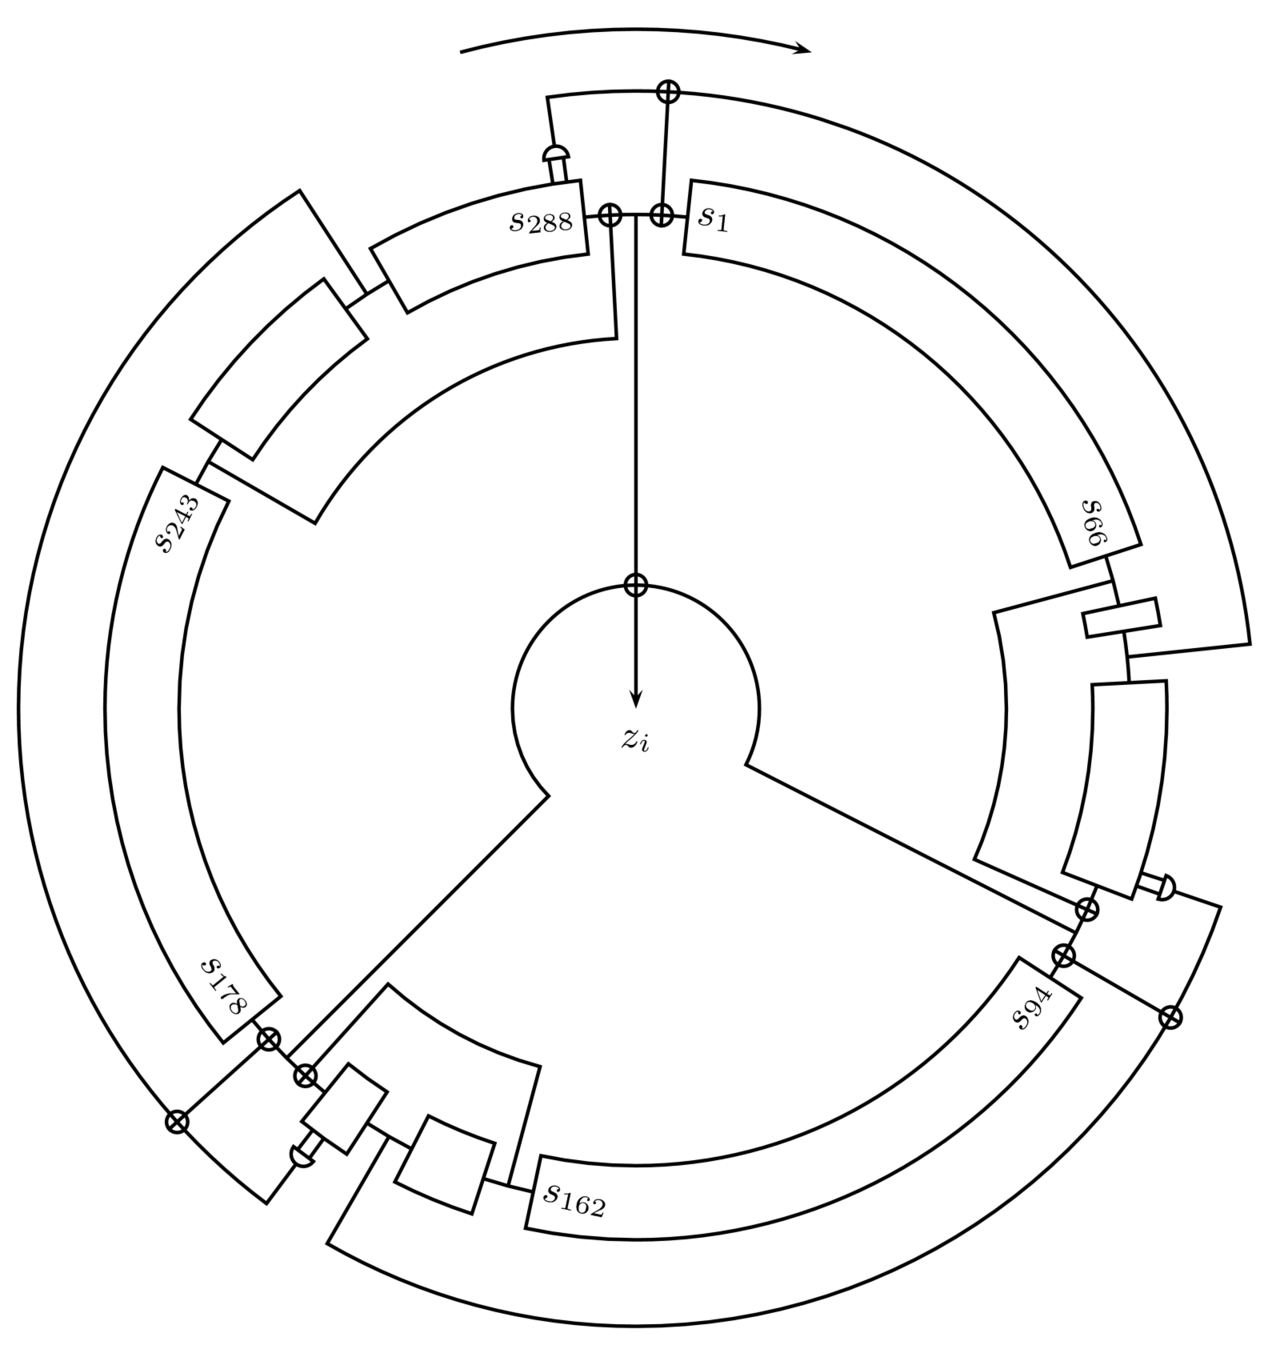
\includegraphics[width=0.45\textwidth]{figures/round.png}
\caption{Trivium \cite{circle}}
\label{fig:circle}
\end{figure}

\subsection{Keystream Generation}\label{sec:key-gen-o}
The keystream is generated as a linear combination of the three registers, $t_1\oplus t_2\oplus t_3=z_i$. At each clock cycle, three bits are update using a non-linear feedback function, whilst one output bit $z_i$ is obtained. The authors state in the cipher specification, that $2^{64}$ keystream bits can be obtained from a given Key/IV pair.

\begin{algorithm}[H]
\begin{algorithmic}[1]
\For{$i=1$ to $N$} \Comment{$N\leq 2^{64}$}
\State $t_1 \gets s_{66} + s_{93}$
\State $t_2 \gets s_{162} + s_{177}$
\State $t_3 \gets s_{243} + s_{288}$
\State
\State $z_i \gets t_1 + t_2 + t_3$
\State
\State $t_1 \gets t_1 + s_{91} \cdot s_{92} + s_{171}$
\State $t_2 \gets t_2 + s_{175} \cdot s_{176} + s_{264}$
\State $t_3 \gets t_3 + s_{286} \cdot s_{287} + s_{69}$
\State
\State $(s_1,s_2,\dots,s_{93}) \gets (t_3,s_1,\dots,s_{92})$
\State $(s_{94},s_{95},\dots,s_{177}) \gets (t_1,s_{94},\dots,s_{176})$
\State $(s_{178},s_{179},\dots,s_{288}) \gets (t_2,s_{178},\dots,s_{287})$
\EndFor
\end{algorithmic}
\caption{Original Keystream Generation}
\end{algorithm}

\subsection{Key and IV Setup}\label{sec:key-iv-o}
The key is loaded into the first eighty bits of the first register, whilst the IV is loaded into the first eighty bits of the second register. All remaining bits are set to zero, with the exception of bits $s_{286},s_{287},s_{288}$ which are set to 1. The instillation stage requires $4*288=1152$ steps and is similar to the keystream generation, except that there are no output bits.

\begin{algorithm}[H]
\begin{algorithmic}[1]
\State $(s_1,s_2,\dots,s_{93}) \gets (K_1,\dots,K_{80},0,\dots,0)$
\State $(s_{94},s_{95},\dots,s_{177}) \gets (IV_1,\dots,IV_{80},0,\dots,0)$
\State $(s_{178},s_{179},\dots,s_{288}) \gets (0,\dots,0,1,1,1)$
\State
\For{$i=1$ to $4\cdot288$}
\State $t_1 \gets s_{66} + s_{91} \cdot s_{92} + s_{93} + s_{171}$
\State $t_2 \gets s_{162} + s_{175} \cdot s_{176} + s_{177} + s_{264}$
\State $t_3 \gets s_{243} + s_{286} \cdot s_{287} + s_{288}+ s_{69}$
\State
\State $(s_1,s_2,\dots,s_{93}) \gets (t_3,s_1,\dots,s_{92})$
\State $(s_{94},s_{95},\dots,s_{177}) \gets (t_1,s_{94},\dots,s_{176})$
\State $(s_{178},s_{179},\dots,s_{288}) \gets (t_2,s_{178},\dots,s_{287})$
\EndFor
\end{algorithmic}
\caption{Original Key and IV Setup}
\end{algorithm}

\begin{figure}[H]
\centering
\includestandalone[width=0.45\textwidth]{figures/original}
\caption{Original Trivium}
\label{fig:original}
\end{figure}

\section{Attack Scenario}


Stuck-at-0 Faults
\begin{itemize}
\item[$\blacktriangleright$] Injecting stuck-at-0 faults can be done in multiple ways.
\begin{itemize}
\item[$\triangleright$] Binary code modification,
\item[$\triangleright$] FPGA bitsream modification,
\item[$\triangleright$] EM fault injection, 
\item[$\triangleright$] Optical fault injection. 
\end{itemize}
\end{itemize}

Assumptions
\begin{itemize}
\item[$\blacktriangleright$] Physical access to device; e.g. during shipment.
\item[$\blacktriangleright$] Proprietary protection mechanism, preventing arbitrary code from being run.
\item[$\blacktriangleright$] Code being executed on device is not signed.
\item[$\blacktriangleright$] Lock bits need to protect against read-back are not set.
\item[$\blacktriangleright$] Key is securely stored and cannot be obtained with ease.
\item[$\blacktriangleright$] Key is reused.
\end{itemize}

Procedure
\begin{itemize}
\item[$\blacktriangleright$] Load fault injected binary onto device.
\item[$\blacktriangleright$] Run fault injected Trivium to obtain $\alpha$ output bits.
\item[$\blacktriangleright$] Cryptanalyse output stream and recover key.
\item[$\blacktriangleright$] Load original binary onto device.
\item[$\blacktriangleright$] Future communications can be deciphered as the key is known.
\end{itemize}


\section{Fault Injection}

\subsection{Keystream Generation}

\begin{algorithm}[H]
\begin{algorithmic}[1]
\For{$i=1$ to $N$} \Comment{$N\leq 2^{64}$}
\State $t_1 \gets s_{66} + s_{93}$
\State $t_2 \gets s_{162} + s_{177}$
\State $t_3 \gets s_{243} + s_{288}$
\State
\State $z_i \gets t_1 + t_2 + t_3$
\State
\State $t_1 \gets t_1 + s_{171}$
\State $t_2 \gets t_2 + s_{264}$
\State $t_3 \gets t_3 + s_{69}$
\State
\State $(s_1,s_2,\dots,s_{93}) \gets (t_3,s_1,\dots,s_{92})$
\State $(s_{94},s_{95},\dots,s_{177}) \gets (t_1,s_{94},\dots,s_{176})$
\State $(s_{178},s_{179},\dots,s_{288}) \gets (t_2,s_{178},\dots,s_{287})$
\EndFor
\end{algorithmic}
\caption{Modified Keystream Generation}
\end{algorithm}

\subsection{Key and IV Setup}

\begin{algorithm}[H]
\begin{algorithmic}[1]
\State $(s_1,s_2,\dots,s_{93}) \gets (K_1,\dots,K_{80},0,\dots,0)$
\State $(s_{94},s_{95},\dots,s_{177}) \gets (IV_1,\dots,IV_{80},0,\dots,0)$
\State $(s_{178},s_{179},\dots,s_{288}) \gets (0,\dots,0,1,1,1)$
\State
\For{$i=1$ to $4\cdot288$}
\State $t_1 \gets s_{66} + s_{93} + s_{171}$
\State $t_2 \gets s_{162} + s_{177} + s_{264}$
\State $t_3 \gets s_{243} + s_{288}+ s_{69}$
\State
\State $(s_1,s_2,\dots,s_{93}) \gets (t_3,s_1,\dots,s_{92})$
\State $(s_{94},s_{95},\dots,s_{177}) \gets (t_1,s_{94},\dots,s_{176})$
\State $(s_{178},s_{179},\dots,s_{288}) \gets (t_2,s_{178},\dots,s_{287})$
\EndFor
\end{algorithmic}
\caption{Modified Key and IV Setup}
\end{algorithm}

\begin{figure}[H]
\centering
\includestandalone[width=0.45\textwidth]{figures/modified}
\caption{Modified Trivium}
\label{fig:modified}
\end{figure}









\section{Code Analysis}

The official C code authored by Christophe De Canni\`ere can be found on  

In the C code the \code{UPDATE()} macro originally does the following
\begin{figure}[H]
\begin{lstlisting}[style=snippet, frame=tlrb]
#define UPDATE()
  do { 
    T(1) = S64(1, 66) ^ S64(1, 93);
    T(2) = S64(2, 69) ^ S64(2, 84);
    T(3) = S64(3, 66) ^ S96(3, 111);

    Z(T(1) ^ T(2) ^ T(3));

    T(1) ^= (S64(1, 91) & S64(1, 92)) ^ S64(2, 78); 
    T(2) ^= (S64(2, 82) & S64(2, 83)) ^ S64(3, 87); 
    T(3) ^= (S96(3, 109) & S96(3, 110)) ^ S64(1, 69); 
  } while (0)
\end{lstlisting}
\caption{Original \code{UPDATE} Macro}
\end{figure}

Performing the modification in the C code will change multiple instructions and the code will not be of the same length as the original.
\begin{figure}[H]
\begin{lstlisting}[style=snippet, frame=tlrb]
#define UPDATE()
  do {
    .       .       .
    .       .       .
    .       .       .
    T(1) ^= S64(1, 91) ^ S64(2, 78); 
    T(2) ^= S64(2, 82) ^ S64(3, 87); 
    T(3) ^= S96(3, 109) ^ S64(1, 69); 
  } while (0)
\end{lstlisting}
\caption{Modified \code{UPDATE} Macro}
\end{figure}















The \code{UPDATE()} macro is used in the \code{ECRYPT\_ivsetup} and \code{ECRYPT\_process\_bytes} functions. This means that when disassembling the \code{trivium.o} object file 

We run the fault injected code using the following key \code{0x0F62B5085BAE0154A7FA} and IV \code{0x288FF65DC42B92F960C7}. Using the Berlekamp–Massey algorithm \cite{massey} we find the shortest linear feedback register (LFSR) for the given bitstream. The polynomial is
$x^{61} + x^{60} + x^{55} + x^{54} + x^{52} + x^{51} + x^{46} + x^{45} + x^{43} + x^{42} + x^{41} + x^{40} + x^{39} + x^{38} + x^{37} + x^{36} + x^{35} + x^{31} + x^{28} + x^{25} + x^{24} + x^{23} + x^{20} + x^{19} + x^{18} + x^{11} + x^8 + x^7 + 1$.

\begin{figure}[H]
\begin{lstlisting}[style=hex, frame=tlrb]
........ EA0421F2 894DBC89 ........ 0FA4F80D
31D121F0 448B65C8 ........ 6DCC440F A4EB1B21
C74431D3 31FB895D ........ 89D30FA4 F30421C3
448B5DC8 ........ E0440FA4 F00921DF 89C34431
........ 13450FA4 E7124121 C74489C0 4131CF45
........ F24589E7  F10E4121 F9448975 C8440FA4
........ 410FA4D7 124121C7 ........  ........
\end{lstlisting}
\caption{Original Binary Code}
\end{figure}

\begin{figure}[H]
\begin{lstlisting}[style=hex, frame=tlrb]
........ EA0433F6 894DBC89 ........ 0FA4F80D 
31D133F6 448B65C8 ........ 6DCC440F A4EB1B33
C04431D3 31FB895D ........ 89D30FA4 F30433C0 
448B5DC8 ........ E0440FA4 F00933C9 89C34431
........ 13450FA4 E71233C0 904489C0 4131CF45
........ F24589E7 F10E33FF 90448975 C8440FA4 
........ 410FA4D7 1233C090 ........  ........
\end{lstlisting}
\caption{Modified Binary Code}
\end{figure}



original
modified
\newcommand{\hf}{\makebox[0pt][l]{\color{green}\rule[-3pt]{0.08\linewidth}{11pt}}}
\newcommand{\ha}{\makebox[0pt][l]{\color{green}\rule[-3pt]{0.04\linewidth}{11pt}}}

\begin{lstlisting}[style=hex, frame=tlrb, escapechar=\%]
1a) ORIG:...    EA0421F2 ........ 31D121F0 ........
1b) MOD:....     EA04%\hf%33F6 ........ 31D1%\hf%33F6  ........

2a)  A4EB1B21 C74431D3 ........ F30421C3
2b)  A4EB1B%\ha%33 %\ha%C04431D3 ........ F304%\hf%33C0

3a) ........ F00921DF ........ E7124121 C74489C0
3b) ........ F009%\hf%33C9 ........ E712%\hf%33C0 %\ha%904489C0 

4a) ........ F10E4121 F9448975 ........ F00D21C8

124121C7
4b) ........ F10E%\hf%33FF %\ha%90448975 ........ F00D33C9

12%\hf%33C0%\ha%90
\end{lstlisting}

A linear system with $k$ variables can be solved in time $k^\omega$, where $\omega \leq 2.376$.
So in our case finding the solution takes at most $288^{2.376} \leq 697,456$ operations


\subsection{Unwinding the bitstream}


\subsection{presentation}


\section{Fault Injection}

\section{Binary Code Modification}

\begin{figure}[H]
\begin{lstlisting}[style=asm, frame=tlrb]
<_ECRYPT_ivsetup>
and    %esi,%edx    21 f2
and    %esi,%eax    21 f0
and    %eax,%edi    21 c7

<_ECRYPT_process_bytes>
and    %eax,%ebx    21 c3
and    %ebx,%edi    21 df  
and    %eax,%r15d   41 21 c7
<...>

and    %edi,%r9d    41 21 f9
<...>
and    %ecx,%eax    21 c8
and    %eax,%r15d   41 21 c7
<...>
\end{lstlisting}
\caption{Original Assembly Code}
\end{figure}

\begin{figure}[H]
\begin{lstlisting}[style=asm, frame=tlrb]
<_ECRYPT_ivsetup>
xor    %esi,%esi    33 f6
xor    %esi,%esi    33 f6
xor    %eax,%eax    33 c0

<_ECRYPT_process_bytes>
xor    %eax,%eax    33 c0
xor    %ebx,%ebx    33 db 
xor    %eax,%eax    33 c0
nop                 90

xor    %edi,%edi    33 ff
nop                 90
xor    %ecx,%ecx    33 c9
xor    %eax,%eax    33 c0
nop                 90
\end{lstlisting}
\caption{Modified Assembly Code}
\end{figure}

\section{Cryptanalysis}

Key from Initial State
\begin{itemize}
\item[$\blacktriangleright$] Express initial state as a system of 288 linear equations.
\item[$\blacktriangleright$] Depends on:
\begin{itemize}
\item[$\triangleright$] 80 unknown bits from key
\item[$\triangleright$] 80 known bits from IV
\item[$\triangleright$] 125 bits set to 0
\item[$\triangleright$] 3 bits set to 1
\end{itemize}
\item[$\blacktriangleright$] A system with $k$ unknown variables can be solved using Gaussian elimination in time $k^\alpha$, where $\alpha\leq 2.376$ \cite{gauss}.
\item[$\blacktriangleright$] Finding the solution takes at most $80^{2.376} \leq 33,247$ operations.
\end{itemize}

Initial State from Keystream
\resizebox{.45\textwidth}{!}{ 
${\displaystyle {\overset {\alpha\times 288{\text{ matrix}}}
{\begin{bmatrix}
a_{1,1}& \dots & a_{1,93} & b_{1,1} & \dots & b_{1,84} & c_{1,1} & \dots & c_{1,111}\\
\vdots &  & \vdots & \vdots &  & \vdots & \vdots &  & \vdots\\
a_{i,1}& \dots & a_{i,93} & b_{i,1} & \dots & b_{i,84} & c_{i,1} & \dots & c_{i,111}\\
\vdots &  & \vdots & \vdots &  & \vdots & \vdots &  & \vdots\\
a_{\alpha,1}& \dots & a_{\alpha,93} & b_{\alpha,1} & \dots & b_{\alpha,84} & c_{\alpha,1} & \dots & c_{\alpha,111}\\
\end{bmatrix}}}
{\overset {288\times 1{\text{ matrix}}}
{\begin{bmatrix}
s_{1} \\
\vdots \\
s_{288} \\
\end{bmatrix}}}
=
{\overset {\alpha\times 1{\text{ matrix}}}
{\begin{bmatrix}
z_{1} \\
\vdots \\
z_{i} \\
\vdots \\
z_{\alpha} \\
\end{bmatrix}}}}
$}

\begin{itemize}
\item[$\triangleright$] $\alpha$ = a time step
\item[$\triangleright$] $a, b, c$ = LFSR 1, 2, 3
\item[$\triangleright$] $s_1,\dots,s_{288}$ = state variables
\item[$\triangleright$] $z_1,\dots,z_{\alpha}$ = output bits
\end{itemize}

\section{Summary}

Summary
\begin{itemize}[itemsep=0.5cm]
\item[$\blacktriangleright$] Stuck-at-0 fault injection attack on binary code.
\item[$\blacktriangleright$] Modify $3 \times 3$ x86 assembly instructions.
\item[$\blacktriangleright$] Injecting stuck-at-0 faults can be done in multiple ways.
\item[$\blacktriangleright$] Reduce the non-linear feedback function to a linear one.
\item[$\blacktriangleright$] The Internal State and Key can be retrieved. 
\end{itemize}

\section*{Acknowledgement}

I would like to thank Elena Dubrova for the idea and her support throughout this project. I'd also like to extend my gratitude towards Per Austrin for making it possible. Daniel Skantz for the invaluable conversations.

\bibliographystyle{IEEEtran}
\bibliography{IEEEabrv,bibl-rep}
\nocite{*}

\end{document}
